\documentclass{article}

\usepackage{fancyhdr}
\usepackage{lastpage}
\usepackage{extramarks}
\usepackage[usenames,dvipsnames]{color}
\usepackage{courier}
\usepackage{amsmath}
\usepackage{amsthm}
\usepackage{amsfonts}
\usepackage{tikz}

\usetikzlibrary{automata,positioning}

\topmargin=-0.45in
\evensidemargin=0in
\oddsidemargin=0in
\textwidth=6.5in
\textheight=9.0in
\headsep=0.25in

\linespread{1.1}

\pagestyle{fancy}
\lhead{\hmwkAuthorName}
\chead{\hmwkClass\ (\hmwkClassInstructor\ \hmwkClassTime): \hmwkTitle}
\rhead{\firstxmark}
\lfoot{\lastxmark}
\cfoot{}
\renewcommand\headrulewidth{0.4pt}
\renewcommand\footrulewidth{0.4pt}

\setlength\parindent{0pt}

\newcommand{\enterProblemHeader}[1]{
    \nobreak\extramarks{#1}{#1 continued on next page\ldots}\nobreak
    \nobreak\extramarks{#1 (continued)}{#1 continued on next page\ldots}\nobreak
}

\newcommand{\exitProblemHeader}[1]{
    \nobreak\extramarks{#1 (continued)}{#1 continued on next page\ldots}\nobreak
    \nobreak\extramarks{#1}{}\nobreak
}

\setcounter{secnumdepth}{0}
\newcounter{homeworkProblemCounter}

\newcommand{\homeworkProblemName}{}
\newenvironment{homeworkProblem}[1][Problem \arabic{homeworkProblemCounter}]{
    \stepcounter{homeworkProblemCounter}
    \renewcommand{\homeworkProblemName}{#1}
    \section{\homeworkProblemName}
    \enterProblemHeader{\homeworkProblemName}
}{
    \exitProblemHeader{\homeworkProblemName}
}

\newcommand{\problemAnswer}[1]{
    \noindent\framebox[\columnwidth][c]{\begin{minipage}{0.98\columnwidth}#1\end{minipage}}
}

\newcommand{\homeworkSectionName}{}
\newenvironment{homeworkSection}[1]{
    \renewcommand{\homeworkSectionName}{#1}
    \subsection{\homeworkSectionName}
    \enterProblemHeader{\homeworkProblemName\ [\homeworkSectionName]}
}{
    \enterProblemHeader{\homeworkProblemName}
}

\newcommand{\hmwkTitle}{Homework\ \#4}
\newcommand{\hmwkDueDate}{February 28, 2013 at 11:59pm}
\newcommand{\hmwkClass}{CS331}
\newcommand{\hmwkClassTime}{9:00am}
\newcommand{\hmwkClassInstructor}{Professor Zhang}
\newcommand{\hmwkAuthorName}{Josh Davis}

\title{
    \vspace{2in}
    \textmd{\textbf{\hmwkClass:\ \hmwkTitle}}\\
    \normalsize\vspace{0.1in}\small{Due\ on\ \hmwkDueDate}\\
    \vspace{0.1in}\large{\textit{\hmwkClassInstructor\ \hmwkClassTime}}
    \vspace{3in}
}

\author{\textbf{\hmwkAuthorName}}
\date{}

\begin{document}

\maketitle

\pagebreak

\begin{homeworkProblem}
    Find a CFG to describe \(L\).
    \\

    The CFG, \(G\), that describes \(L\) is below:

    \[
        G = (V, \Sigma, R, S)
    \]

    such that

    \[
        G = (\{A, B\}, \{a, b, c\}, R, A)
    \]
    where

    \[
        \begin{split}
            R: &
            \\
               & A \rightarrow aAc | B | \epsilon
            \\
               & B \rightarrow bB | \epsilon
        \end{split}
    \]

    The push down automata that represents \(G\) is as follows:

    \begin{figure}[here]
        \centering
        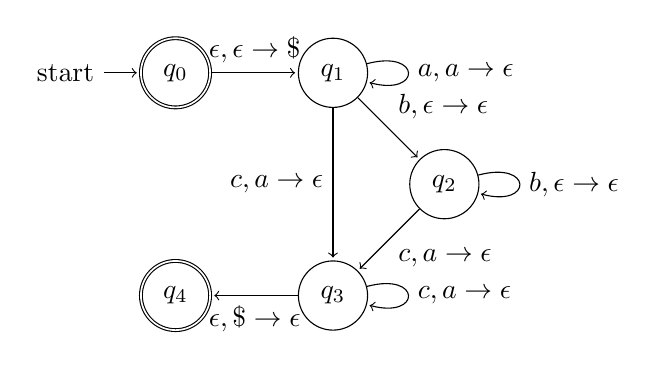
\begin{tikzpicture}[shorten >=1pt,node distance=2cm,on grid,auto] 
            \node[state, initial, accepting] (q_0) {$q_0$}; 
            \node[state] (q_1) [right=of q_0] {$q_1$}; 
            \node[state] (q_2) [below right=of q_1] {$q_2$}; 
            \node[state] (q_3) [below left=of q_2] {$q_3$}; 
            \node[state, accepting] (q_4) [left=of q_3] {$q_4$}; 
            \path[->] 
                (q_0)
                    edge node {$\epsilon, \epsilon \rightarrow \$ $} (q_1)
                (q_1)
                    edge [loop right] node {$a, a \rightarrow \epsilon $} (q_1)
                    edge node [left] {$c, a \rightarrow \epsilon $} (q_3)
                    edge node {$ b, \epsilon \rightarrow \epsilon $} (q_2)
                (q_2)
                    edge [loop right] node {$b, \epsilon \rightarrow \epsilon $} (q_2)
                    edge node {$ c, a \rightarrow \epsilon $} (q_3)
                (q_3)
                    edge [loop right] node {$c, a \rightarrow \epsilon $} (q_2)
                    edge node {$\epsilon, \$ \rightarrow \epsilon $} (q_4)
                    ;
        \end{tikzpicture}
        \caption{PDA, \(A\)}
        \label{fig:automataA}
    \end{figure}

\end{homeworkProblem}

\pagebreak

\begin{homeworkProblem}
    \textbf{Part A}
    \\
    Prove that if \(L\) is context-free and \(L'\) is a regular languagte, then
    \(L \cap L'\) is context-free too.
    \\
    
    \begin{proof}
        If \(L\) is a context-free language, and \(L'\) is a regular language, then
        let \(M\) and \(N\) be the finite automata and push down automata that
        accept both languages respectively.
        \\

        We can construct a new push down automata, \(O\) such that \(M\) and
        \(N\) both receive the input and the new machine accepts a word only if
        both \(M\) and \(N\) accept it. This is possible because a finite
        automata doesn't use a stack which means one stack is sufficient for
        the complete push down automata. This concludes the proof.
    \end{proof}

    \textbf{Part B}
    \\
    Let \(\Sigma = \{a, b, c\}\) and
    \[
        L = \{ w \in \Sigma^* : w \mbox{ contains equal number of a's, b's, and c's} \}
    \]

    Prove that \(L\) is not a context-free language.

    \begin{proof}
        Suppose \(L\) is context-free. Let \(L' = \{a^* b^* c^*\}\), a regular language.
        \\

        Then according to what we proved in the first part, \(L \cap L'\) is
        context-free. This is a contradiction because the language \(\{a^n b^n
        c^n\}\) is not context-free thus violating our previous proof. We have
        arrived at a contradiction therefore our proof is complete.

    \end{proof}

\end{homeworkProblem}

\pagebreak

\begin{homeworkProblem}
    Prove that right linear grammars recognize exactly the class of regular languages.

    \begin{proof}
        This proof will consist of two parts. First proving that any regular
        language can be described by a RLG, and that any language described by
        an RLG is regular.
        \\

        \textbf{Part One}
        Proving that any regular language can be described by an RLG.
        \\

        Let \(G = \langle V, \Sigma, R, S \rangle\), a right linear grammar. We can construct a
        NFA, \(A = (Q, \Sigma, \delta, q, F)\) as follows:

        \begin{enumerate}
            \item \(Q = \{v : \mbox{ for every } v \in V\}\)
            \item The alphabet is the same, \(\Sigma = \Sigma\)
            \item The start state is the start variable, \(q = S\)
            \item Since a grammar is complete once all variables are removed, we can add a new
                final state for this, \(F = V_{final}\)
            \item For every rule, there is a transition from the variable state, \(S\) to the next
                variable state, \(T\). Since it is a right linear grammar, for every rule there exists a
                rule such that \(S \rightarrow wT\), where \(w \in \Sigma^*\). Therefore we can represent the transition from one
                variable state to the next as a string of states such that there is a state for every
                terminal character in the rule. For example, the rule \(S \rightarrow abT\) would be represented
                as follows:
                \begin{figure}[here]
                    \centering
                    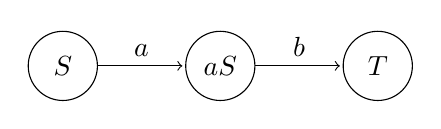
\begin{tikzpicture}[shorten >=1pt,node distance=2cm,on grid,auto] 
                        \node[state] (S) {$S$}; 
                        \node[state] (a) [right=of S] {$aS$}; 
                        \node[state] (T) [right=of a] {$T$}; 
                        \path[->] 
                            (S)
                                edge node {$a$} (a)
                            (a)
                                edge node {$b$} (T);
                    \end{tikzpicture}
                \end{figure}
        \end{enumerate}

        This shows that our right linear grammar, \(G\) can be made into an automata, \(A\).
        \\

        \textbf{Part Two}
        Proving that any language described by an RLG is regular.
        \\

        Let \(A = (Q, \Sigma, \delta, q, F)\), a finite automata. We can construct a right
        linear grammar similar to how we constructed an NFA above. We will construct a
        RLG, \(G = \langle V, \Sigma, R, S \rangle\) as follows:

        \begin{enumerate}
            \item \(V = \{q : \mbox{ for every } q \in Q\}\)
            \item The alphabet is the same, \(\Sigma = \Sigma\)
            \item The start variable becomes the start state, \(S = q\)
            \item For every transition, \(\delta(q, a) = q_1\) where \(q_1 \in Q\), we can create a rule for it such that
                \(R\) would be defined as follows:
                \[
                    \begin{split}
                        R: &
                        \\
                           & q \rightarrow aq_1
                    \end{split}
                \]
        \end{enumerate}

        This shows that any finite automata can be made into a right linear grammar.
        \\

        Since both sides have been proven, the proof is complete and RLGs
        recognize exactly the class of regular languages.

    \end{proof}
\end{homeworkProblem}

\pagebreak

\begin{homeworkProblem}
    Use pumping lemma to show that the following language is not context-free:
    \[
        L = \{a^i b^j c^k : i, j, k \geq 0 \mbox{ and } i > j \mbox{ and } j > k \}
    \]

    \begin{proof}
        We let \(w = a^{p + 2} b^{p + 1} c^{p}\) where \(p\) is the pumping length.
        We then split up \(w\) so that \(w = uvxyz\). In doing so, we can break it up into
        cases like so:
        \begin{enumerate}
            \item \(vxy\) contains just a's. This will result in a contradiction
                because pumping down yields \(a^{0} a^{p - 2} a^{0} = \epsilon a^p \epsilon\) which means \(i \leq j\) and
                thus \(w \notin L\).
            \item \(vxy\) contains just b's. This will result in a contradiction
                because pumping down yields \(b^{0} b^{p - 2} b^{0} = \epsilon b^p \epsilon\) which means \(j \leq k\) and
                thus \(w \notin L\).
            \item \(vxy\) contains just c's. This will result in a contradiction
                because pumping up will eventually give us \(k > j\)
                thus \(w \notin L\).
            \item \(vxy\) is the split between a's and b's. 
                This can be divided into four more cases:
                \begin{enumerate}
                    \item \(vxy = aab\), pumping down will lower the number of b's to be the same as
                        the number of c's. Thus \(w \notin L\).
                    \item \(vxy = abb\), pumping down will lower the number of a's to be the same as
                        the number of b's. Thus \(w \notin L\).
                    \item \(vxy = \epsilon ab\), pumping up will increase the number of b's past the
                        number of a's. Thus \(w \notin L\).
                    \item \(vxy = ab \epsilon\), pumping down will lower the number of a's to be the
                        same as the number of b's. Thus \(w \notin L\).
                \end{enumerate}

            \item \(vxy\) is the split between b's and c's. Regardless of where the subsplit is,
                it can be pumped until eventually \(i < j\) or \(i < k\), thus \(w \notin L\).
        \end{enumerate}
        
        Now that I have (hopefully) exhausted all possibilities, the proof is complete and the language,
        \(L\), is not context-free.
    \end{proof}
\end{homeworkProblem}

\pagebreak

\begin{homeworkProblem}
    Let \(G = \langle \{S\}, \{a, b\}, R, S \rangle\) be a context-free grammar
    with the rules, \(R\) defined as follows:
    \[
        S \rightarrow aS | aSbS | \epsilon
    \]

    \textbf{Part One}
    Prove that \(G\) is ambiguous.
    \\
    \begin{proof}
        We can prove that \(G\) is ambiguous if there are two left most derivations
        for one string.
        \\

        Take \(s = aab\), it can be derived twice as follows:
        \[
            \begin{split}
                S &= aS = aaSbS = aabS = aab
                \\
                S &= aSbS = aaSbS = aabS = aab
            \end{split}
        \]
        
        Thus the context free language, \(G\) is ambiguous.
    \end{proof}

    \textbf{Part Two}
    Give unambigous grammar that generates the same language as \(G\).
    \\

    The new grammar can be defined as follows:
    \[
        \begin{split}
            S &\rightarrow aT | T
            \\
            T &\rightarrow aSbU | S
            \\
            U &\rightarrow a | b | \epsilon
        \end{split}
    \]

    Using the previous example of \(s = aab\), we can try to derive it multiple times
    like so:
    \[
        \begin{split}
            S &= aT = aSbU = aTbU = aabU = aab
            \\
            S &= T = aSbU = ... = \mbox{ no way to get aab}
        \end{split}
    \]

    And there it can't be derived multiple ways. So unless I'm missing
    something, I think the homework is finished. YAY!
    
\end{homeworkProblem}

\end{document}
